%%
%% This is file `sample-xelatex.tex',
%% generated with the docstrip utility.
%%
%% The original source files were:
%%
%% samples.dtx  (with options: `sigconf')
%% 
%% IMPORTANT NOTICE:
%% 
%% For the copyright see the source file.
%% 
%% Any modified versions of this file must be renamed
%% with new filenames distinct from sample-xelatex.tex.
%% 
%% For distribution of the original source see the terms
%% for copying and modification in the file samples.dtx.
%% 
%% This generated file may be distributed as long as the
%% original source files, as listed above, are part of the
%% same distribution. (The sources need not necessarily be
%% in the same archive or directory.)
%%
%% Commands for TeXCount
%TC:macro \cite [option:text,text]
%TC:macro \citep [option:text,text]
%TC:macro \citet [option:text,text]
%TC:envir table 0 1
%TC:envir table* 0 1
%TC:envir tabular [ignore] word
%TC:envir displaymath 0 word
%TC:envir math 0 word
%TC:envir comment 0 0
%%
%%
%% The first command in your LaTeX source must be the \documentclass command.
\PassOptionsToPackage{table}{xcolor}
\documentclass[sigconf,nonacm]{acmart}
%% NOTE that a single column version is required for 
%% submission and peer review. This can be done by changing
%% the \doucmentclass[...]{acmart} in this template to 
%% \documentclass[manuscript,screen]{acmart}
%% 
%% To ensure 100% compatibility, please check the white list of
%% approved LaTeX packages to be used with the Master Article Template at
%% https://www.acm.org/publications/taps/whitelist-of-latex-packages 
%% before creating your document. The white list page provides 
%% information on how to submit additional LaTeX packages for 
%% review and adoption.
%% Fonts used in the template cannot be substituted; margin 
%% adjustments are not allowed.

%%
%% \BibTeX command to typeset BibTeX logo in the docs
\AtBeginDocument{%
  \providecommand\BibTeX{{%
    \normalfont B\kern-0.5em{\scshape i\kern-0.25em b}\kern-0.8em\TeX}}}

%% Rights management information.  This information is sent to you
%% when you complete the rights form.  These commands have SAMPLE
%% values in them; it is your responsibility as an author to replace
%% the commands and values with those provided to you when you
%% complete the rights form.
% \setcopyright{acmcopyright}
% \copyrightyear{2018}
% \acmYear{2018}
% \acmDOI{XXXXXXX.XXXXXXX}

%% These commands are for a PROCEEDINGS abstract or paper.
% \acmConference[Conference acronym 'XX]{Make sure to enter the correct
%   conference title from your rights confirmation emai}{June 03--05,
%   2018}{Woodstock, NY}
%
%  Uncomment \acmBooktitle if th title of the proceedings is different
%  from ``Proceedings of ...''!
%
%\acmBooktitle{Woodstock '18: ACM Symposium on Neural Gaze Detection,
%  June 03--05, 2018, Woodstock, NY} 
% \acmPrice{15.00}
% \acmISBN{978-1-4503-XXXX-X/18/06}

\usepackage[table]{xcolor}
\usepackage{array}
\usepackage{xeCJK}
\setCJKmainfont[AutoFakeBold=true, AutoFakeSlant=true]{標楷體}

\newcolumntype{P}[1]{>{\raggedright\vrule height4ex width 0pt}p{#1}<{\vrule depth 2.5ex width 0pt}}


%%
%% Submission ID.
%% Use this when submitting an article to a sponsored event. You'll
%% receive a unique submission ID from the organizers
%% of the event, and this ID should be used as the parameter to this command.
%%\acmSubmissionID{123-A56-BU3}

%%
%% The majority of ACM publications use numbered citations and
%% references.  The command \citestyle{authoryear} switches to the
%% "author year" style.
%%
%% If you are preparing content for an event
%% sponsored by ACM SIGGRAPH, you must use the "author year" style of
%% citations and references.
%% Uncommenting
%% the next command will enable that style.
%%\citestyle{acmauthoryear}
%%
%% end of the preamble, start of the body of the document source.
\begin{document}

%%
%% The "title" command has an optional parameter,
%% allowing the author to define a "short title" to be used in page headers.
\title{Accelerate Canny Edge Detector with Parallel Programming}

%%
%% The "author" command and its associated commands are used to define
%% the authors and their affiliations.
%% Of note is the shared affiliation of the first two authors, and the
%% "authornote" and "authornotemark" commands
%% used to denote shared contribution to the research.
\author{Zi Yi Huang}
\affiliation{
  \institution{312551072}
  \institution{IOC, NYCU}
  \city{Hsinchu}
  \country{Taiwan}
}
\email{m312551072.cs12@nycu.edu.tw}

\author{Bo Han Chen}
\affiliation{
  \institution{312551074}
  \institution{IOC, NYCU}
  \city{Hsinchu}
  \country{Taiwan}
}
\email{bhchen312551074.cs12@nycu.edu.tw}

\author{Hsuan Yu Chi}
\affiliation{
  \institution{312551080}
  \institution{IOC, NYCU}
  \city{Hsinchu}
  \country{Taiwan}
}
\email{chihy.cs12@nycu.edu.tw}

%%
%% By default, the full list of authors will be used in the page
%% headers. Often, this list is too long, and will overlap
%% other information printed in the page headers. This command allows
%% the author to define a more concise list
%% of authors' names for this purpose.
% \renewcommand{\shortauthors}{Trovato and Tobin, et al.}

%%
%% The abstract is a short summary of the work to be presented in the
%% article.
% \begin{abstract}
  
% \end{abstract}

%%
%% The code below is generated by the tool at http://dl.acm.org/ccs.cfm.
%% Please copy and paste the code instead of the example below.
%%
% \begin{CCSXML}
% <ccs2012>
%  <concept>
%   <concept_id>00000000.0000000.0000000</concept_id>
%   <concept_desc>Do Not Use This Code, Generate the Correct Terms for Your Paper</concept_desc>
%   <concept_significance>500</concept_significance>
%  </concept>
%  <concept>
%   <concept_id>00000000.00000000.00000000</concept_id>
%   <concept_desc>Do Not Use This Code, Generate the Correct Terms for Your Paper</concept_desc>
%   <concept_significance>300</concept_significance>
%  </concept>
%  <concept>
%   <concept_id>00000000.00000000.00000000</concept_id>
%   <concept_desc>Do Not Use This Code, Generate the Correct Terms for Your Paper</concept_desc>
%   <concept_significance>100</concept_significance>
%  </concept>
%  <concept>
%   <concept_id>00000000.00000000.00000000</concept_id>
%   <concept_desc>Do Not Use This Code, Generate the Correct Terms for Your Paper</concept_desc>
%   <concept_significance>100</concept_significance>
%  </concept>
% </ccs2012>
% \end{CCSXML}

% \ccsdesc[500]{Do Not Use This Code~Generate the Correct Terms for Your Paper}
% \ccsdesc[300]{Do Not Use This Code~Generate the Correct Terms for Your Paper}
% \ccsdesc{Do Not Use This Code~Generate the Correct Terms for Your Paper}
% \ccsdesc[100]{Do Not Use This Code~Generate the Correct Terms for Your Paper}

%%
%% Keywords. The author(s) should pick words that accurately describe
%% the work being presented. Separate the keywords with commas.
% \keywords{Do, Not, Us, This, Code, Put, the, Correct, Terms, for,
%   Your, Paper}

%% A "teaser" image appears between the author and affiliation
%% information and the body of the document, and typically spans the
%% page.
% \begin{teaserfigure}
%   \includegraphics[width=\textwidth]{sampleteaser}
%   \caption{Seattle Mariners at Spring Training, 2010.}
%   \Description{Enjoying the baseball game from the third-base
%   seats. Ichiro Suzuki preparing to bat.}
%   \label{fig:teaser}
% \end{teaserfigure}

% \received{20 February 2007}
% \received[revised]{12 March 2009}
% \received[accepted]{5 June 2009}

%%
%% This command processes the author and affiliation and title
%% information and builds the first part of the formatted document.
\maketitle

\section{Introduction}
  Canny Edge Detection (CED) 是一種常見的影像處理演算法,用於偵測圖片中的大範圍邊界。
  它是在1986年由John F. Canny發明。Canny Edge Detection可以有效地去除影像中的雜訊、
  模糊的邊緣與非邊緣的線,產生更高SNR的影像,使結果更為精細。
  以下是Canny Edge Detection常見的應用領域 (1) Object detection : 偵測影像中物體的邊緣,
  用於辨識物體。如用於偵測道路交通中的汽車、行人和其他物體。(2) Image segmentation : 
  將影像分割成不同的圖像子區域,用於進一步分析。實際可應用於醫學影像、指紋識別、人臉識別等 
  (3) Feature extraction : 從影像中提取特徵,提取物體的邊緣或建築物的角落。
  這些功能隨後可用於物件辨識。如從臉部影像提取特徵進行人臉識別,或從街道影像中提取特徵用於自動駕駛。
  結合以上應用,因此Canny Edge Detection在醫學圖像分析、機器人學、電腦視覺、
  工業檢驗相關研究領域廣泛使用。 \\
  Canny Edge Detection的優點可以分為以下幾點
  \begin{enumerate}
    \item Accurate edge localization : 可以精準的定位圖片中的邊緣,確保僅保留重要的邊緣
    \item Low error rate : 演算法中double thresholding 與 edge tracking的機制降低誤判邊緣的可能性,
    因此有較低錯誤率。
    \item Single response to edges : 圖片中每條邊緣在輸出僅由single response表示,
    避免重複邊緣偵測,使線條更為細緻。
    \item Robust to noise : 適用於受到各種噪聲影響的真實世界圖片影像。
    起始步驟中的Smoothing使Canny Edge Detection具有很高的抗噪性。
  \end{enumerate}
  缺點則是
  \begin{enumerate}
    \item Computationally expensive : Canny Edge Detection的計算成本很高,尤其圖片解析度很高時。
    \item Sensitive to parameters : double thresholding的選擇會很大程度影響邊緣偵測的輸出結果,
    對於不同圖片會有適合的threshold。
  \end{enumerate}
  Canny Edge Detection的計算成本相當高,包含多個卷積、
  Gradient Computation、Nonmaxima Suppression、BFS搜尋。雖然複雜,
  但計算間有獨立性,可使用平行處理來加速。透過將影像劃分為多個區域,使用thread
  平行處理每個區域,在多核心處理器上加速;或使用GPU矩陣乘法來加速卷積運算。
  藉由平行運算,可以在不影響正確性的情形下提升計算效率與throughput,滿足需要處理大量資料的需求。

\section{Statement of Problem}

在這個部分,我們會介紹 Canny Edge Detection 演算法,描述演算法中各步驟的運作,
最後分析哪些部分是可以使用平行化來加速的。
Canny Edge Detection 演算法分成以下幾個步驟:Smoothing、Gradient Computation、
Nonmaxima Suppression、Double Thresholding 和 Hysteresis Edge Linking,
接下來我們會針對每個步驟做詳細的說明。

\subsection{Smoothing} \label{Smoothing}

對於 Smoothing,我們使用一個 $3\times3$ 的近似高斯濾波器 $G$ 來對輸入的影像進行卷積,
以達到平滑影像的效果。
$$G=\frac{1}{16}
\begin{bmatrix}
1 & 2 & 1 \\2 & 4 & 2 \\
1 & 2 & 1
\end{bmatrix}$$
令 $f(x, y)$ 為輸入影像,則經過 Smoothing 後的影像 $f_s(x, y)$ 可以表示為 $f$ 與 $G$ 的卷積,
如下算式所示:
$$f_s(x, y)=f(x, y)*G(x, y)$$

\subsection{Gradient Computation}

對於 Gradient Computation,我們需要計算上一步中得到的 $f_s(x, y)$ 上每個點的梯度大小與方向,
我們使用 Sobel filter 來計算梯度,Sobel filter 有兩種,分別是 $S_x$ 與 $S_y$,
分別代表用來計算水平與垂直方向的梯度的 filter,如下所示:
$$S_x=\begin{bmatrix} -1 & 0 & 1 \\ -2 & 0 & 2 \\ -1 & 0 & 1 \\ \end{bmatrix} S_y=\begin{bmatrix} -1 & -2 & -1 \\ 0 & 0 & 0 \\ 1 & 2 & 1 \\ \end{bmatrix}$$
水平方向及垂直方向的梯度分別計算如下:
\begin{align*}
  g_x(x, y)=f_s(x, y)*S_x(x, y)\\
  g_y(x, y)=f_s(x, y)*S_y(x, y)
\end{align*}
接著計算每個點上的梯度大小 $M(x, y)$,以及其梯度方向 $\alpha(x, y)$,
其中 $M(x, y)$ 為梯度的 Euclidean vector norm,$\alpha(x, y)$ 為梯度的方向,計算如下列算式所示:
$$M(x, y)=||\nabla f(x, y)||=\sqrt {{g_x}^2(x, y)+{g_y}^2(x, y)}$$
$$\alpha(x, y)=\text{tan}^{-1}(\frac{g_y(x, y)}{g_x(x, y)})$$

\subsection{Nonmaxima Suppression} \label{NMS}

在計算完  $f_s(x, y)$ 上每個點的梯度大小與方向後,我們使用 Nonmaxima Suppression 對邊緣進行細化,
Nonmaxima Suppression 後的圖片表示為 $f_N(x, y)$。對 $M(x, y)$ 的每個點,
我們尋找一個最接近其梯度方向 $\alpha(x, y)$ 的方向 $d_k$ 
(在我們的方法中我們分成 4 個方向,分別是水平、垂直、左上到右下、右上到左下),
並將 $M(x, y)$ 與兩鄰居的梯度大小 $M(x-\Delta x, y-\Delta y)$ 及 $M(x+\Delta x, y+\Delta y)$ 
(以下表示為 $M_a, M_b$) 做比較,其中 $\Delta x$ 與 $\Delta y$ 為 $d_k$ 的水平與垂直方向的位移量,
比較的結果有兩種情況,如果 $M(x, y)$ 比兩鄰居都大,則 $f_N(x, y)=M(x, y)$,
反之 $f_N(x, y)=0$,如下算式所示:
$$f_N(x, y)=\begin{cases} M(x, y) & \text{if } M(x, y) \geq M_a \text{ and } M(x, y) \geq M_b
 \\ 0 & \text{otherwise} \end{cases}$$
\begin{align*}
  M_a=M(x-\Delta x, y-\Delta y) \\ M_b=M(x+\Delta x, y+\Delta y)
\end{align*}

\subsection{Double Thresholding}

在計算完 $f_N(x, y)$ 後,接著對 $f_N(x, y)$ 中所有點做 Double Thresholding,
High threshold 與 Low threshold 的值表示為 $T_h$ 與 $T_l$,
我們將 $f_N(x, y)$ 中的點分成三類,分別是 strong pixel, 
weak pixel 和 non-relevant pixel,分別表示為為 edge、可能為 edge、不是 edge的 pixel,
分別定義如下:

\begin{itemize}
  \item strong pixel: $M(x, y) \geq T_h$
  \item weak pixel: $T_h > M(x, y) \geq T_l$
  \item non-relevant pixel: $M(x, y) < T_l$
\end{itemize}

\subsection{Hysteresis Edge Linking}

在得到 $f_N(x, y)$ 中的 strong pixel 與 weak pixel 後,
我們將所有 strong pixel 排入 queue,對 queue 中每個點的 8-connected component 做 BFS,
將連通的 weak pixel 設為 strong pixel,並將其排入 queue,直到 queue 為空為止,
最後得到的圖片即為 Canny Edge Detection 的結果。

\subsection{Why we choose this problem?}

這個演算法因為是應用在影像上的,且需要對圖片中每個像素做計算,需要大量的時間,
但觀察演算法的這幾個步驟,可以發現許多步驟中都需要使用 for 迴圈遍歷整張圖片的所有像素,
且在同一個步驟中,遍歷的過程中每個像素的計算都是獨立的,因此我們可以將這些步驟平行化,
以加速演算法的執行,下一個章節我們將介紹我們計畫如何將這些步驟平行化。

\section{Proposed Approaches}

這個部份我們會詳細介紹如何將CED中的各個步驟利用Pthread、OpenMP和CUDA進行平行化,
並在不影響邊緣偵測正確性的同時加速原本的CED演算法。

\subsection{Smoothing}

此步驟利用\ref{Smoothing}所提到的濾波器對圖像進行卷積抑制原圖中的噪音;由於卷積運算是各像素獨立進行,
因此可以利用Pthread和CUDA將各像素的運算交由thread,使用CPU和GPU加速。
另外我們也會使用OpenMP對原程式中的for loop進行CPU加速,並和Pthread、CUDA的結果進行比較。

\subsection{Gradient Calculation}

藉由Sobel filter計算圖像中各像素的梯度和向量角度時,因為是各像素獨立運算,
所以運算之間不具有資料相依性;我們同樣利用Pthread和CUDA將不同像素運算分派給不同thread,
使用CPU和GPU加速;OpenMP的部分也是對原程式中的for loop進行CPU加速。

\subsection{Nonmaxima Suppression}

為了限縮上述邊緣厚度至單一像素的大小,我們會依據各像素與其鄰居的梯度值和向量角度,
判斷該像素是否為潛在的邊緣像素。由於此方法的運算是基於前一步驟的結果,因此運算之間並無資料相依性的問題。
我們可以使用不同thread判斷不同像素是否為該向量方向的最大值,並結合Pthread和CUDA,
利用CPU和GPU加速完成平行化。
由於此步驟在線性運算時會使用for迴圈進行運算,因此我們也會使用OpenMP,利用CPU達到平行度。

\subsection{Double Thresholding}

此步驟藉由\ref{NMS}所提到的兩個閥值,$T_h$和$T_l$,判斷NMS所得出的像素為strong、weak或non-relevent pixel。
由於此步驟為各像素間的獨立運算,因此我們一樣會使用Pthread和CUDA進行多線程的運算;
迭代運算的部分可以使用OpenMP進行加速。

\subsection{Hysteresis Edge Linking}

為了尋找出最後的邊緣像素,我們先將strong pixel存在queue中,
再利用BFS將連接strong pixel的weak pixel納入CED的最終邊緣結果。
為了達成平行化,我們會使用Pthread將圖像分割給不同thread進行BFS運算,
在thread清空各自的queue後,將該圖像分區的邊緣辨識結果寫回各thread之間共享的記憶體。
不過這樣的做法會在圖像分割的邊界出現weak pixel沒有被標示為strong pixel的情形,
因此需要在分割時讓各thread負責的區域重疊1 像素的寬度,
當全部的thread完成寫入後再針對重疊區域進行BFS運算。
在使用CUDA進行此步驟的平行化時,我們依據Luo等人在\cite{4563088}提出的方法,將圖像分割給不同的thread block,
並由thread block中的thread進行BFS運算;雖然同一block中的thread可以達成同步,
但thread block之間無法進行同步,因此我們會使用論文中所提出的multi-pass方式重複進行數次BFS運算,
避免相鄰區域的邊緣結果無法連結。

\subsection{Parallelization Strategies}

綜上所述,我們會將CED的平行化分為For Loop Parallelism和Data Decomposition兩部分,
前四步驟為將各像素的運算交由thread進行加速,Hysteresis Edge Linking的部分則是將圖像分割,
讓thread對各分區進行運算。流程圖如圖\ref{fig:diagram}所示。

\begin{figure}[h]
  \centering
  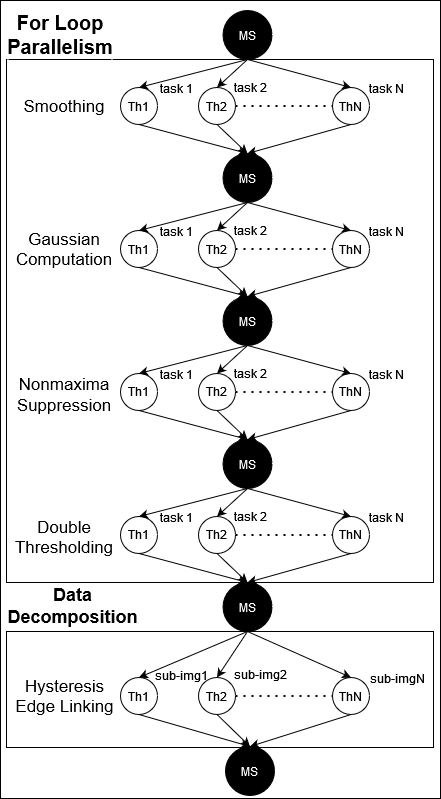
\includegraphics[width=\linewidth]{parallel_diagram.png}
  \caption{Parallel Strategies and Flow Chart of Canny Edge Detection Parallelism}
  \label{fig:diagram}
\end{figure}

\section{Language Selection}

我們的程式語言使用 C++。因為C++ 是編譯型語言,在執行之前會被轉換為機器碼,
使C++ 較為快速和高效;且C++ 提供控管記憶體的方式,給予一定靈活與設計空間;
同時C++ STL提供多種 API 來支持平行化,包括std::future、std::atomic等。
並且可使用其他框架來支持平行化,如OpenMP、CUDA、OpenCL。

\section{Related Work}

Gonzalez等人在 \cite{gonzalez2018digital} 中提及了 Canny 演算法的概念,
並介紹了每個步驟中的過程並給出了一些實做細節上的選擇,比如 Smoothing 中 filter 的選擇,
或是 Gradient Computation 中計算 Gradient 的方式,但沒有提及如何使用平行化加速演算法的執行,
所以我們接下來將介紹其他將此演算法利用平行化加速的研究。\\
Cheikh等人在\cite{6328953}中提出了兩種平行化的策略,
分別為loop-level parallelism和domain decomposition;
loop-level parallelism是將個步驟中可獨立運行的迴圈交由多個thread執行,
但由於需要反覆進行fork-join,因此會有額外的開銷,
且會因為計算全域資料而失去資料局部性(data locality);
domain decomposition是將資料本身進行分割再交由thread完成各分區的各項步驟,
雖然domain decomposition沒有前述loop-level parallelism的缺陷,
但需要選擇適合的資料分割方式來降低平行化時的相依性來達到最佳效能。
Cheikh等人將兩種方式在多核CPU和GPU上進行實驗,
發現loop-level parallelism在GPU上運行無serial的程式時可以達到很好的加速效果,
而domain decomposition適合在CPU上針對大型資料的運算進行平行化;
最後他們結合了兩種平行化策略,發現結合後的加速效果和擴展性相比於兩種平行化策略,
在CPU和GPU的表現都更好,因此我們在針對CED的平行化策略上,
也採取了結合loop-level parallelism和domain decomposition的方式,預期可以達到最好的成果。 \\
Luo等人在在\cite{4563088}中嘗試以CUDA 框架對Canny Edge Detection進行平行化,
並且提到過往在Canny Edge Detection中hysteresis labeling connected component part的平行化處理較少,
因為此步驟平行化需要non-local memory,導致速度與效率顯著降低。
論文中使用GPU在處理pixel-wise operations有較高效率的特性來加速non-maximum suppression、
hysteresis and connected components等部分,並引入Apron pixels的機制來讓所有像素可以在卷積中操作。
實驗結果顯示,與CPU版本的實作相比,隨著圖片大小而有1.6X\~3.8X不等的加速效果。
另外GPU版本的hysteresis為了同步不同thread block間的運算使用了multi-pass approach,
導致GPU運算速度降低,佔據75\%以上的運行時間。

\section{Statement of Expected Results}

針對CED的平行化,我們提出了數個理論並希望可以藉由實驗來觀察並驗證其正確性。

\subsection{圖像大小 vs. 加速效果}

我們會針對不同大小的圖像進行CED的平行化測試,由於CED的多個步驟都是針對各像素進行運算,
可以推斷圖像大小等同於運算量的多寡,因此我們預期大張圖像的加速效果會優於小張圖像的加速效果。

\subsection{平行化程式的擴展性}

藉由不同的thread數量進行實驗,我們可以計算在運行多個thread的情況下是否可以達到預期的加速效果。
因為Hysteresis Edge Linking步驟需要對thread進行同步,
因此我們認為該步驟會在增加thread的同時增加同步所需要的開銷,從而限制加速的效果。

\subsection{Pthread vs. OpenMP}

雖然Pthread和OpenMP同樣使用CPU進行加速,但針對thread的行為部分,
Pthread是開發者自定義而OpenMP是取決於編譯器,因此我們認為Pthread的加速效果會優於OpenMP。

\subsection{Pthread vs. CUDA}

CUDA雖然使用GPU進行加速,但需要將資料在記憶體和GPU之間進行搬運,從而增加搬運的開銷;
因此我們會利用小張圖像測試Pthread和CUDA的加速效果,
觀察搬運開銷是否會在運算小張圖像時降低CUDA的加速效果。

\subsection{Comparison of All Method}

最後我們會利用1920*1080的圖像對不同加速方法進行測試,觀察並比較不同方法之間的加速效果。

\section{Timetable}

下表為我們的進度排程
\begin{table*}[h]
  \begin{tabular}{|P{5cm}*{9}{|c}|}
    \hline
    \centering \raisebox{-2ex}[0pt][0pt]{Action plan} & \multicolumn{4}{c|}{Nov} & \multicolumn{4}{c|}{Dec} \\
    \cline{2-9}
    \multicolumn{1}{|c|}{\vphantom{$\Big|$}} &
    \scriptsize W1 & \scriptsize W2 & \scriptsize W3 & \scriptsize W4 &
    \scriptsize W1 & \scriptsize W2 & \scriptsize W3 & \scriptsize W4 \\
    \hline
    Serial Program of CED &
    \multicolumn{2}{c}{\cellcolor{gray}} &&&&&& \\
    \hline
    Pthread and OpenMP Parallelism &
    && \multicolumn{2}{c}{\cellcolor{gray}} &&&& \\
    \hline
    CUDA Parallelism &
    &&&& \multicolumn{2}{c}{\cellcolor{gray}} && \\
    \hline
    Experiment \& Evaluation  &
    &&& \multicolumn{4}{c}{\cellcolor{gray}} & \\
    \hline
    Final Report and \\ Presentation Preparation &
    &&&&&&& \multicolumn{1}{c}{\cellcolor{gray}}  \\
    \hline
  \end{tabular}
\end{table*}

%%
%% The next two lines define the bibliography style to be used, and
%% the bibliography file.
\bibliographystyle{ACM-Reference-Format}
\bibliography{sample-base}

\end{document}
\endinput
%%
%% End of file `sample-xelatex.tex'.
